%=========================================================================
% sec-parallel-node
%=========================================================================

\subsection{Parallelizing for the Compute Node}
\label{sec-parallel-node}

A relatively simple way to parallelize work in any structured grid
computation, including the shallow water equation solver in this
assignment, is to divide the grid into blocks and assign each thread a
block for which to compute the solution. We will refer to the cells in
this block as \emph{live cells}. Depending on the stencil radius of the
computation kernel, we also need a ring of padding cells called
\emph{ghost cells} that are consumed in order to calculate the solution
for the boundary cells of the block. Here we redefine a \emph{block} as
the live cells and ghost cells required by a thread to calculate the
solutions for all of the live cells. We say 'consume' since after
advancing a timestep, an additional outermost \texttt{r} layers of the
ghost cell ring become obsolete, where \texttt{r} is the stencil
radius. The radius of the ring of ghost cells we need depends on the
number of timesteps we want each thread to execute before synchronizing
(i.e., updating the ghost cells with new solutions from other
threads). Executing more than one timestep before synchronization is
referred to as \emph{batching} and will be discussed in
Section~\ref{sec-tune}. For this section, we assume each thread only
executes a single timestep before synchronization.

In order to apply the blocking parallelization to the shallow water
equation solver, we first need to identify which functions can or cannot
be parallelized in the computation kernel. \texttt{Central2D::run()}
calls the following functions:

\begin{itemize}
  \item \texttt{apply\_periodic()}
  \item \texttt{compute\_fg\_speeds()}
  \item \texttt{limited\_derivs()}
  \item \texttt{compute\_step()}
\end{itemize}

The \texttt{apply\_periodic()} function updates the ghost cells of the
grid by copying the outermost \texttt{r} layers of the live cells
in a periodic fashion, where \texttt{r} is the ghost cell radius. This
function forces a synchronization point since the ghost cells in a given
block depend on the live cells of other blocks, meaning each thread has
to communicate the solutions of the live cells in its block to all of the
other threads. As such, this function only needs to be called at the
beginning of every super-step (i.e., main computation sub-step +
staggered computation sub-step).

The \texttt{compute\_fg\_speeds()} function is actually comprised of two
separate logical functions: (1) calculating the maximum wave speeds in
the x/y directions, and (2) updating the flux vectors. (1) is only used
to calculate the \texttt{dt} which does not change within a super-step
and uses expensive square root operations, so we separate this into a
\texttt{compute\_wave\_speeds()} function that is called once before
every super-step. This function is similar to \texttt{apply\_periodic()}
in that it requires synchronization across threads, in this case to
calculate the maximum wave speeds across all blocks in the grid, thus
making it difficult to parallelize naively. On the other hand, (2) still
needs to be called at every sub-step, but can independently calculate the
\texttt{f} and \texttt{g} vectors for a block without synchronization.

The \texttt{limited\_derivs()} function calculates the \texttt{ux},
\texttt{uy}, \texttt{fx}, and \texttt{gy} vectors from the \texttt{u},
\texttt{f}, and \texttt{g} vectors to implement the \texttt{MinMod}
limiter. The \texttt{compute\_step()} function then uses these output
vectors to calculate the solution vectors, \texttt{u}, for the current
timestep. These functions can also independently calculate the output
vectors without synchronization.

%=========================================================================
% fig-parallel-node-blocking.tex
%=========================================================================

\begin{figure}[h]

  \centering
  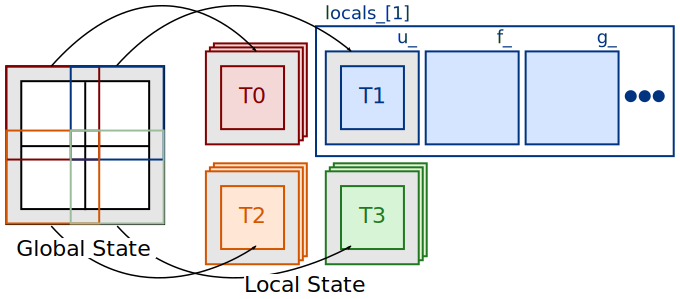
\includegraphics[width=0.9\tw]{fig-parallel-node-blocking.svg.pdf}

  \caption{\textbf{Parallelizing Computation Using Per-Thread Local State --}
    In this example, the global grid is divided into four local blocks,
    each of which is copied to per-thread memory allocated separately
    from the global grid. The LocalState class encapsulates all vectors
    in a local block including \texttt{u\_}, \texttt{f\_}, \texttt{g\_},
    \texttt{ux\_}, \texttt{uy\_}, \texttt{fx\_}, \texttt{gy\_}, and
    \texttt{v\_}. Each thread is only responsible for computing the
    solution of the live cells (i.e., non-gray area) in its local
    block. In order to do so, the vectors in the ghost cells (i.e., gray
    area) must be used. Note that the ghost cells of one local block
    overlap with the live cells of other local blocks grid, causing
    redundant computation. }

  \label{fig-parallel-node-blocking}

\end{figure}


For now, we apply the blocking parallelization to the
\texttt{compute\_flux()}, \texttt{limited\_derivs()}, and
\texttt{compute\_step()} functions and leave parallelization of the other
functions for future optimizations. Because the ghost cells of each block
become contaminated with incorrect vectors and ghost cells of one block
overlap with live cells of other blocks, it is important that we
allocate per-thread memory for storing various vectors of the block
separate from the \emph{global} state. As such, we encapsulate this
per-thread information in a class called \texttt{LocalState} that holds
the vectors for the \emph{local} state: \texttt{u\_}, \texttt{f\_},
\texttt{g\_}, \texttt{ux\_}, \texttt{uy\_}, \texttt{fx\_}, \texttt{gy\_},
and \texttt{v\_}. In fact, all of these vectors with the exception of
\texttt{u\_} are only used in the local state computation; we only need
to keep a separate global state for
\texttt{u\_}. Figure~\ref{fig-parallel-node-blocking} shows a visual
representation of how the global grid is divided into local blocks. A
vector of pointers to per-thread \texttt{LocalState} objects is kept as a
member variable of \texttt{Central2D} called \texttt{locals\_} that can
be indexed by the thread ID.

To facilitate copying of vectors between the global and local states, we
implement the \texttt{copy\_to\_local()} and \texttt{copy\_from\_local()}
functions. Note that these functions can easily be parallelized since
copying to the local state only has conflicting accesses on reads, and
copying from the local state only writes the live cells in the global
grid which do not overlap between local blocks. The ghost cells of the
global grid are updated by the \texttt{apply\_periodic()} function.

The pseudocode for our current parallelization is as follows:

\begin{verbatim}
  while (t < tfinal) {
    apply_periodic();
    real dt = calculate_dt(compute_wave_speed());
    #pragma omp parallel num_threads(nthreads)
    {
      int tid = omp_get_thread_num();
      copy_to_local(tid);
      for (int io : sub_steps) {
        compute_flux(tid);
        limit_derivs(tid);
        compute_step(tid);
      }
      copy_from_local(tid);
    }
    t = update_time(dt);
  }
\end{verbatim}

%=========================================================================
% fig-parallel-node-results.tex
%=========================================================================

\begin{figure}[h]

  \begin{minipage}[t]{0.48\tw}
  \begin{subfigure}{\tw}

  \centering
  \includegraphics[width=1.0\tw]{fig-parallel-node-strong-results.py.pdf}
  \caption{\textbf{Strong Scaling Study}}
  \label{fig-parallel-node-strong-results}

  \end{subfigure}
  \end{minipage}%
  \hfill%
  \begin{minipage}[t]{0.48\tw}
  \begin{subfigure}{\tw}

  \centering
  \includegraphics[width=1.0\tw]{fig-parallel-node-weak-results.py.pdf}
  \caption{\textbf{Weak Scaling Study}}
  \label{fig-parallel-node-weak-results}

  \end{subfigure}
  \end{minipage}%

  \caption{\textbf{Performance Results of Parallel Implementation of
      Shallow Water Equation Solver Running on Compute Nodes --}
    Performance of the parallel implementation of the shallow water
    equation solver running on the Totient compute nodes compared against
    the tuned serial implementation for all initial conditions. All
    speedups are the execution time normalized to the serial
    implementation. For the strong scaling experiment, we use an 800x800
    grid.  For the weak scaling study, we start the baseline at 200x200
    and increase the problem size at the same factor as the increasing number
    of threads (e.g., 200x200 grid for 1 thread, 400x400 grid for 4 threads, etc.). }

  \label{fig-parallel-node-results}

\end{figure}



The preliminary results comparing the performance of the serial and
parallel implementations of the shallow water equation solver running the
compute nodes is shown in Figure~\ref{fig-parallel-node-results}.

For the strong scaling study, we sweep the number of threads used for the
parallel implementation using the same 800x800 grid size and normalize
the execution time results against the serial implementation. In prior results the general
theme was a pseudo-linear speedup with the number of threads until 6
threads, then the performance tapered off with any additional increase in
parallelization, and was using a 200x200 grid. This is to be expected, especially with a smaller
dataset, since the synchronization overhead begins to dominate the amount
of work per thread with more threads.

In comparing with the tuned code, however, we do not see the kinds of speedup
we would like for the parallel implementation.  We believe the reason for this is
two-fold. First, there is suboptimal load balancing for block dimensions
that do not evenly divide the grid dimensions -- less work will be assigned to the
boundary blocks. Second, there might be an increase in cache conflicts
for certain block dimensions. This effect would be most noticeable during
the copying of data to and from the per-thread local state, which occurs
after every timestep. The interplay between this effect and the fact that
smaller blocks are more likely to fit in each thread's (i.e., core's)
private L1 cache, could be a possible cause of the inconsistency we see
for the performance of certain block dimensions.

Furthermore, the rate at which our \texttt{LocalState<Physics>} class requires new data
to be initialized at each execution of the \texttt{Sim::run} method provides for a sizeable
overhead.  A better choice would have been to re-use as much memory as possible.

For the weak scaling study, we increase the grid size with the same
factor as the increase in the number of threads. For example, the 4
thread configuration uses a 400x400 grid, whereas the serial
configuration uses a 200x200 grid. An ideal weak scaling parallel
implementation would have a roughly constant speedup for increasing
numbers of threads. These studies help programmers to identify the impact
of synchronization overheads in their parallel implementations. In our
results, we see an approximate exponential decay in performance as we
scale the problem size with the number of threads, implying that our
synchronization overhead does not scale linearly with the number of
threads. However, it is important to keep in mind that this trend is
likely partly due to the fact that increasing the grid dimensions
increases the computational complexity by an order of $N^3$, rather than
$N^2$. This is because we are not only increasing the total number of
elements on the grid, but we are also increasing the total number of
timesteps required to compute a single frame (i.e., requires more
timesteps to reach convergence for a larger grid). Since we are
increasing the number of timesteps, it is natural that the number of
synchronization boundaries between timesteps increase as well.


